\documentclass[12pt,a4paper]{article}
\usepackage[latin1]{inputenc}
\usepackage{float}
\usepackage{amsmath}
\usepackage{amsfonts}
\usepackage{amssymb}
\usepackage{graphicx}
\usepackage[hidelinks]{hyperref}
\usepackage{changepage}
\usepackage{subfig}
\usepackage{placeins}



\author{Davide Cocco - 944122\\
	Marco Gasperini - 944922}
\date{A.Y. 2019/2020 - Prof. Di Nitto Elisabetta}


\title{
	\textbf{\Huge{SafeStreets}} \\
	\large Design Document
}

\begin {document}

	\begin{figure}
		\centering
		
\includegraphics[width=1.0\linewidth]{Images/polimi.jpg}
	\end{figure}

	\maketitle
	\newpage
	\tableofcontents
	\newpage

\section{INTRODUCTION}
\subsection{Purpose}
This \texttt{Design Document (DD)} for the SafeStreets software will provide a functional description of the system by describing its architecture. 
It will eventually by used by the development team as a blueprint to guide the engineering of the application.
\subsection{Scope}
The main objective of the S2B will be assisting (thus not substituting) authorities and officers in handling traffic violations though a crowd-sourced platform in which civilians can participate. 
A mobile application will allow users, both civilians and officers, to report violations through the use of the camera and the GPS, sending the data to authorities who will process such reports. 
Law enforcement will be aided by a data mining system which will produce relevant data about the registered violations, and the S2B will be able to automatically compile a ticket and send it to
the municipality's VLA as soon as an officer personally convalidates a violation.
\subsection{Definitions, Acronyms, Abbreviations}
\subsubsection{Definitions}
\begin{itemize}
\item \texttt{Violation | Offence:} we will strictly refer to any kind of static traffic violation, especially parking violations. 
\item \texttt{Authority:} a law enforcement authority which is manages traffic violations, it could be the local police, the traffic wardens etc. We will refer with this term also to the personnel which operates the web application in the authorities' headquarters.
\item \texttt{User:} refers to the users of the mobile application, that is officers and civilians.
\end{itemize}
\subsubsection{Acronyms}
\begin{itemize}
\item \texttt{S2B:} software to be.
\item \texttt{HFVZ:} high violation frequency zone.
\item \texttt{GPS:} Global Positioning System.
\item \texttt{GDPR:} General Data Protection Regulation.
\item \texttt{DW:} data warehouse.
\item \texttt{VLA:} Vehicle Licensing Authority.
\item \texttt{RACS:} Reliable Array of Cloned Services.
\item \texttt{RAPS:} Reliable Array of Partitioned Services.
\item \texttt{GUI:} Graphical User Interface.
\item \texttt{DMZ:} Demilitarized zone.
\item \texttt{ADS:} Application and Data server of the authorities.
\end{itemize}
\subsubsection{Abbreviations}
\begin{itemize}
	\item {[Gn]}: n-goal.
	\item {[Rn]}: n-requirment.
	\item {[Dn]}: n-domain assumption
	\item {App}: application.
\end{itemize}
\subsection{Revision History}
\subsection{Reference Documents}
\subsection{Document Structure}
\begin{itemize}
\item \textbf{Introduction}: includes the purpose and scope of the document along with some relevant definitions and acronyms used throughout the document.
\item \textbf{Architectural design}: this section is focused on the main components used for this system and the relationship between them, providing information about their
deployment and how they operate. it also focuses on the architectural styles and the design patterns adopted for designing the system.
\item \textbf{User interface design}: this section provides an overview on how the User Interface will look like, but it will be omitted due to the presence of this chapter in the RASD.
\item \textbf{Requirements traceability}: in this sections the requirements highlighted in the RASD document will be associated with the design elements explained in this document.
\item \textbf{Implementation, integration and test plan}: in this section we identify the order in which we plan to implement the subcomponents of the system and the order in which we plan to
integrate and test them.
\end{itemize}
\newpage
\section{ARCHITECTURAL DESIGN}
\subsection{High level overview}
			\begin{figure}[H]
				\centering
					\begin{adjustwidth}{-25mm}{-25mm}
					        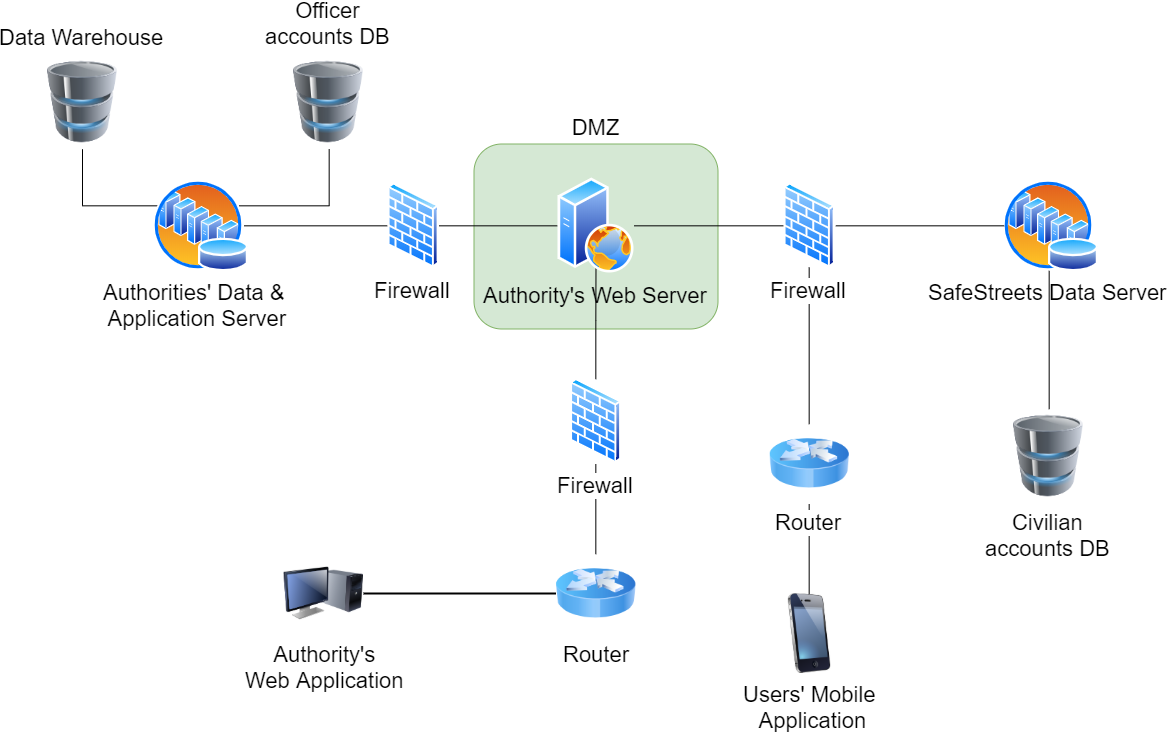
\includegraphics[width=.9\paperwidth,keepaspectratio]{Images/highlevel}
					\end{adjustwidth}
				\caption{Figure 1: High Level Structure with a single Authority and a single User}
			\end{figure}
The three logical layers of the S2B can be seen in different ways depending on the actor's client, as different actors can access different services. From the \textbf{Authority's perspective} we can see the layers distributed in a \textbf{two-tier architecture}:
\begin{itemize}
\item \textbf{Presentation layer:} the GUI at the authority's web application is the tool thanks to which the authority's personnel can add officers, receive reports  from the users through HTTP calls thanks to a REST architecture embedded in the web server, and validate or invalidate them. It can thus interact 
with the Application and Data server (we will call it ADS from now on) to which it sends validated reports and receives updates, the users' clients, and rarely with the SafeStreets' server to which it sends ban requests. The web server is isolated from the outside by firewalls for increased security and to protect the ADS even if the web server is compromised.
\item \textbf{Application and Data layer:} the ADS manages application functionalities such as ticket emission and update spreading, and also data functionalities such as managing the officers' accounts in an ad-hoc database and
enriching a standalone data warehouse with reports to be processed. This server's location can either be in a central authority location for reduced latency, a municipality etc. and can be replicated through a RAPS architecture, (e.g. every authority can have its own server)
to be able to handle multiple requests in settings like big cities. 
\end{itemize}

From the \textbf{Civilian's perspective} we can see the layers distributed in a \textbf{three-tier architecture}:
\begin{itemize}
\item \textbf{Presentation layer:} the GUI at the mobile application, which can be used to file reports and send them to the Authority's web server. 
\item \textbf{Application layer:} the hypermedia at the mobile application moves from a state to another thanks to the updates received by the authorities' web servers (which are themselves sent to the authorities by their application server), that are periodically spread to the clients in the network. 
This is done to avoid having the clients know the application and data servers' access points. This way the mobile application can only contact one of the authorities' web servers and all the report processing and updating procedures are black boxed from the users perspective.
\item \textbf{Data layer:} the data server at the SafeStreets headquarters, which can be replicated through a RACS architecture to be simply scalable, manages civilian accesses and bans.
\end{itemize}

From the \textbf{Officer's perspective} we have a similar perspective as the civilian's, but officers' accounts are managed by the authorities' Application and Data server, thus we can see the layers distributed in a \textbf{two-tier architecture}:
\begin{itemize}
\item \textbf{Presentation layer:} the GUI at the mobile application which possesses the same features as the civilians' one but also includes the abilities to check a report and sign the automated ticket by inserting the officer's secret PIN, and also receives slightly different updates which
include sensitive data to be made unreadable by civilians. 
\item \textbf{Application and Data layer:} just as the civilians' perspective but in this case accounts are managed in the same location where the application functionalities resiede (as officers account aren't located in the DB at SafeStreets headquarters) and thus the application and data layers are merged.
Officers, just as civilians, only communicate directly with one of the city's authorities' web server which then handles interacting with the Application and Data server to provide the functionalities.
\end{itemize}

It is important to denote the fact that since every Authority owns a web server, calls received from the mobile units can be handled by any of the authorities for load balancing. The only logic which will be implemented at the authorities' client will be the supervised algorithm to recognize plates: this way
we can reduce latency, because since the overhead to effectively send a correct plate frame will be pretty heavy, we remove the step to contact the application server and instead execute this function directly at the authorities' location. Anything else will be handled as notifications forwarded to the ADS
to limit the computational power used at the authorities' locations.


\subsection{Component view}
The following diagrams illustrate the system components and the interfaces through which they interact to fullfil their functionalities. The diagram is focused on the application tier, so the remaining tiers (the presentation tier and the data tier) are shown as black-box.
First we have done a distinction between Client side and Server side:
\begin{itemize}
\item The Client side is composed by two components, \textit{Web Application} and \textit{Mobile Application}. The first is referred to the Authorities client, latter to the User client (Civilian and Officer).
\item The Server side is composed of three main components: \textit{Authorities Web Services} manages the authorities client, through the \textit{AuthoritiesWebServices} interface server-side; the other two services are the \textit{Civilian Mobile Services} and the \textit{Officer Mobile Services} that manage  the \textit{Mobile Application} from two distinct interfaces.
\end{itemize}
\begin{figure}[H]
		\centering
			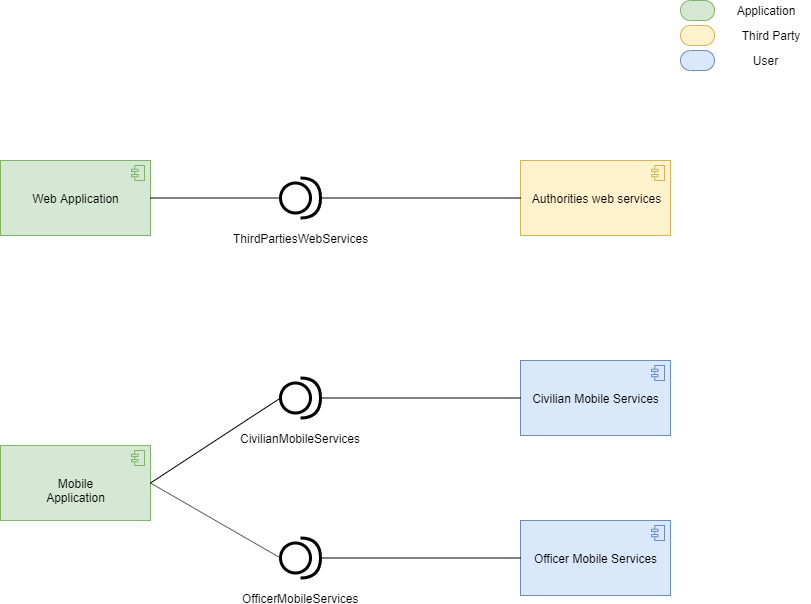
\includegraphics[width=1.0\linewidth]{Images/ComponentDiagram}
		\caption{Figure 2: Component diagram}
\end{figure}

\subsection{Deployment view}
\subsection{Runtime view: You can use sequence diagrams to describe the way components interact to accomplish specific tasks typically related to your use cases}
\subsection{Component interfaces}
\subsection{Selected architectural styles and patterns: Please explain which styles/patterns you used, why, and how}
\subsection{Other design decisions}
\section{USER INTERFACE DESIGN: Provide an overview on how the user interface(s) of your system will look like; if you have included this part in the RASD, you can simply refer to what you have already done, possibly, providing here some extensions if applicable.}
\section{REQUIREMENTS TRACEABILITY: Explain how the requirements you have defined in the RASD map to the design elements that you have defined in this document.}
\section{IMPLEMENTATION, INTEGRATION AND TEST PLAN: Identify here the order in which you plan to implement the subcomponents of your system and the order in which you plan to integrate such subcomponents and test the integration.}
\section{EFFORT SPENT}
\begin{itemize}
\item {Davide Cocco}
 \begin{center}
			\begin{tabular}{| c | l | c |}
				\hline
				\textbf{Day} & \textbf{Subject} & \textbf{Hours} \\ \hline
				Total & & 22.5 \\ \hline
			\end{tabular}
		\end{center}
\item {Marco Gasperini}
\begin{center}
			\begin{tabular}{| c | l | c |}
				\hline
				\textbf{Day} & \textbf{Subject} & \textbf{Hours} \\ \hline
				Total & & 19.5 \\ \hline
			\end{tabular}
\end{center}
\end{itemize}
\section{References}

\end {document}